\section{Architettura del sistema NeuroFrame}
Analizziamo ora l'architettura dell'intero sistema NeuroFrame scendendo di livello.\newline
La \emph{figura 3.1} in questa sezione espande quanto visto ad alto livello nella \emph{figura 2.2}.
\vspace{5mm}
\begin{figure}[H]
  \centering
  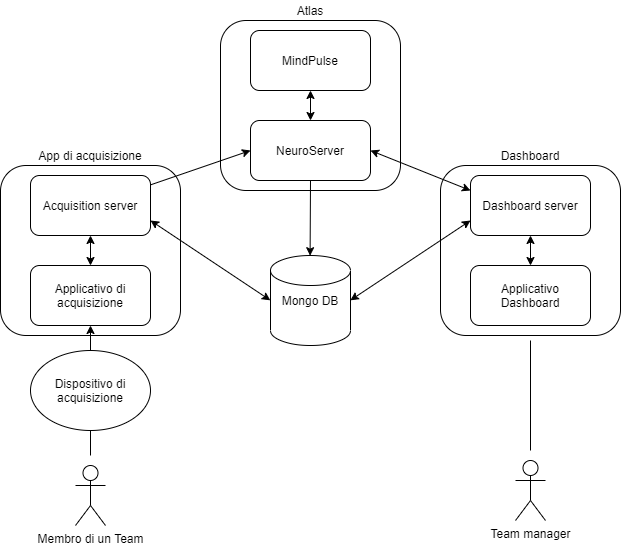
\includegraphics[width=0.85\textwidth]{img/NeuroFrameCompleto.png}
  \caption{Archittettura completa del sistema distribuito NeuroFrame}
\end{figure}
\noindent Qui ritroviamo la nota struttura interna della {\bf piattaforma Atlas}, costituita dal {\bf NeuroServer} e dagli \emph{algoritmi di elaborazione} (in figura per semplicità è indicato l'unico algoritmo rilevante nel sistema NeuroFrame, cioè {\bf MindPulse}).\newline

\noindent Anche lato Acquisizione e Dashboard troviamo una divisione analoga; {\bf per ogni endpoint vi è un applicativo usato dagli utenti finali ed un server dedicato}.
I server comunicano tra loro ed utilizzano il database come snodo centrale per condividere dati persistenti.\newline

\noindent Riprendendo il flusso informativo lato Dashboard, discusso nella \emph{sezione 2.2.3}, possiamo vedere in \emph{figura 3.2} come esso rimanga sostanzialmente invariato se non per il fatto che vi è un passaggio extra dato dal server (la situazione è analoga lato Acquisizione, che il cui diagramma di sequenza non viene riportato per evitare eccessiva ridondanza).
\vspace{5mm}
\begin{figure}[H]
  \centering
  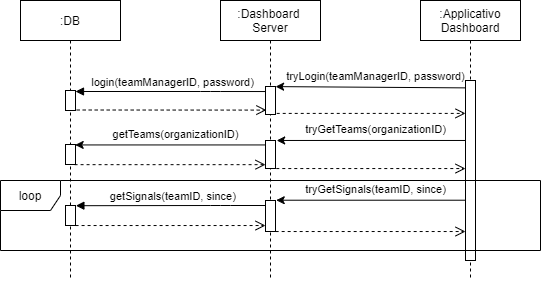
\includegraphics[width=1.0\textwidth]{img/diagramma_sequenza_dashboard_completo.png}
  \caption{Diagramma di sequenza rappresentante il flusso informativo completo lato Dashboard}
\end{figure}
\vspace{5mm}
\noindent Vediamo ora le {\bf scelte tecnologiche e strutturali legate al database}.

\subsection{Storage dei dati: utilizzo di database non relazionali}
Il database scelto per NeuroFrame è di tipo {\bf non relazionale}, in particolare si è optato per l'utilizzo di {\bf MongoDB} \cite{what_is_mongoDB}.\newline
La scelta è stata dettata dalle caratteristiche del mezzo che ben si sposano con le esigenze di Vibre e del progetto.\newline

\noindent In primo luogo la motivazione più importante che ha portato a tale scelta è da attribuirsi alla grande {\bf flessibilità} offerta da MongoDB; questa caratteristica ricopre un ruolo fondamentale all'interno di un progetto in rapido mutamento.\newline
Se difatti un classico database relazionale SQL offre dei vincoli che rendono la consistenza dei dati molto solida, le stesse limitazioni mal si sposano con l'evolversi di nuove feature (dettate anche dal feedback dei clienti) e delle strutture dati stesse (specialmente in vista delle evoluzioni degli algoritmi neurali della piattaforma Atlas, in particolare dell'algoritmo MindPulse in questo contesto).\newline

\noindent MongoDB inoltre utilizza documenti {\bf JSON-like}, un formato semplice da usare che negli ultimi anni si sta rapidamente affermando come standard de facto, specialmente in ambito web.\newline 

\noindent Ultimo motivo, non meno importante, è la capacità di MongoDB di {\bf eseguire interrogazioni e manipolazioni dei dati lato DB molto più potenti e complesse} rispetto ad un database relazionale SQL.
\subsubsection{Struttura del database}
Di seguito sono esposte le \emph{collezioni} che compongono il database MongoDB dedicato al sistema NeuroFrame, nonché la \emph{struttura interna} di ciascuna di esse.\newline

\noindent{\bf Organizations}\newline
Collezione dedicata allo storage delle organizzazioni che utilizzano il servizio.
\begin{itemize}
  \item \emph{organization id}\\
  {Identificativo, univoco per ogni organizzazione.}
  \item \emph{logo}\\
  {URI preposto al recupero del logo dell'organizzazione.}
  \item \emph{teams}\\
  {Array contenente gli identificativi dei Team presenti nell'organizzazione.}
  \item \emph{team managers}\\
  {Array contenente gli identificativi dei Team managers presenti nell'organizzazione.}
  \item \emph{users}\\
  {Array contenente gli identificativi degli Utenti presenti nell'organizzazione.}
  \item \emph{license}\\
  {Struttura volta ad indicare i dati relativi al tipo di licenza acquistata (si vedano vincoli definiti nella sezione \emph{2.2.4}).}
  {\begin{itemize}
    \item \emph{name}\\
    {Tipologia di licenza acquistata.}
    \item \emph{max users per team}\\
    {Numero massimo di Utenti \emph{per ogni Team} consentito dal tipo li licenza acquistata.}
    \item \emph{max teams}\\
    {Numero massimo di Team \emph{nell'Organizzazione} consentito dal tipo di licenza acquistata.}
  \end{itemize}}
\end{itemize}

\noindent{\bf Team managers}\newline
Qui vengono memorizzati tutti i Team manager esistenti.
\begin{itemize}
  \item \emph{user id}\\
  {Identificativo, univoco \emph{all'interno della stessa Organizzazione}.}
  \item \emph{organization id}\\
  {Riferimento all'identificativo dell'Organizzazione di cui il Team manager fa parte.}
  \item \emph{password}\\
  {Password del Team manager.}
\end{itemize}

\noindent{\bf Users}\newline
Collezione preposta alla memorizzazione degli Utenti presenti in NeuroFrame.
\begin{itemize}
  \item \emph{user id}\\
  {Identificativo dell'Utente, \emph{univoco all'interno della stessa Organizzazione}.}
  \item \emph{organization id}\\
  {Riferimento all'Organizzazione di cui l'Utente fa parte.}
  \item \emph{password}\\
  {Password dell'Utente.}
  \item \emph{current team}\\
  {Riferimento all'identificativo del Team di cui l'Utente fa parte al momento (vuoto se non fa parte di un Team).}
\end{itemize}

\noindent{\bf Teams}\newline
Spazio dove saranno memorizzati i dati relativi a tutti i Team.
\begin{itemize}
  \item \emph{team id}\\
  {Identificativo del Team, \emph{univoco all'interno dell'Organizzazione}.}
  \item \emph{organization id}\\
  {Riferimento all'identificativo dell'organizzazione che ha creato il Team.}
  \item \emph{users}\\
  {Array contentente gli identificativi degli Utenti facenti parte del Team.}
\end{itemize}

\noindent{\bf Signals}\newline
Collezione chiave per il funzionamento di NeuroFrame. Contiene tutte le metriche elaborate dalla piattaforma Atlas.\newline
Ogni entry all'interno della collezione contiene un numero massimo di misurazioni, date delle limitazioni imposte sulle dimensioni dei dati da MongoDB. Una stessa acquisizione di segnali neurali dunque, dipendentemente dalla sua durata temporale, può essere divisa in più parti; ogni parte corrisponde a singole entry di questa collezione.
\begin{itemize}
  \item \emph{user id}\\
  {Riferimento all'identificativo dell'Utente a cui le metriche fanno capo.}
  \item \emph{organization id}\\
  {Riferimento all'identificativo dell'Organizzazione a cui l'Utente appartiene.}
  \item \emph{team id}\\
  {Riferimento al Team di cui l'Utente era membro \emph{nel momento dell'acquisizione} (è possibile che il Team manager sposti l'Utente in un altro Team).}
  \item \emph{data}\\
  {Array contenente dati strutturati ordinati temporalmente.}
  {\begin{itemize}
    \item \emph{fatigue}\\
    {Metrica rappresentante l'affaticamento mentale dell'individuo (\emph{sezione 1.1}).}
    \item \emph{workload}\\
    {Metrica rappresentante il carico cognitivo dell'individuo (\emph{sezione 1.1}).}
    \item \emph{timestamp}\\
    {Istante temporale del campionamento.}
  \end{itemize}}
  \item \emph{start}\\
  {Corrisponde al timestamp del primo elemento dell'array data.}
  \item \emph{end}\\
  {Corrisponde al timestamp dell'ultimo elemento dell'array data.}
\end{itemize}